\documentclass[a4paper, 12pt]{article}
\usepackage[english]{babel}
\usepackage[numbers]{natbib}
\usepackage{url}

\def\UrlBreaks{\do\A\do\B\do\C\do\D\do\E\do\F\do\G\do\H\do\I\do\J
\do\K\do\L\do\M\do\N\do\O\do\P\do\Q\do\R\do\S\do\T\do\U\do\V
\do\W\do\X\do\Y\do\Z\do\[\do\\\do\]\do\^\do\_\do\`\do\a\do\b
\do\c\do\d\do\e\do\f\do\g\do\h\do\i\do\j\do\k\do\l\do\m\do\n
\do\o\do\p\do\q\do\r\do\s\do\t\do\u\do\v\do\w\do\x\do\y\do\z
\do\.\do\@\do\\\do\/\do\!\do\_\do\|\do\;\do\>\do\]\do\)\do\,
\do\?\do\'\do+\do\=\do\#}


\usepackage[utf8x]{inputenc}
\usepackage{amsmath}
\usepackage{graphicx}
\graphicspath{{figures/}}
\usepackage{parskip}
\usepackage{fancyhdr}
\usepackage{vmargin}
\usepackage{float}
\setmarginsrb{2.5 cm}{2.5 cm}{2.5 cm}{2 cm}{1 cm}{1 cm}{1 cm}{1.5 cm}

\title{\Large Deep NMT Off-line Deployment in Mobile Devices}     % Title
\author{Yilin Zheng\\Shupei Chen\\Chenxuan Wang}                               % Author
\date{\today}                                           % Date

\makeatletter
\let\thetitle\@title
\let\theauthor\@author
\let\thedate\@date
\makeatother

\pagestyle{fancy}
\fancyhf{}
\rhead{Yilin et al.}
\lhead{Deep MNT Off-line Deployment in Mobile Devices}
\cfoot{\thepage}

\begin{document}

\begin{titlepage}
    \centering
    \vspace*{0.5 cm}
    
\includegraphics[scale = 0.4]{sustech_logo.png}\\[1.0 cm]   % University Logo
    \textsc{\Large Southern University of Science and Technology}\\[1.5 cm]   % University Name
    \textsc{\Large CS322}\\[0.5 cm]               % Course Code
    \textsc{\large Innovative Experiment II}\\[0.5 cm]               % Course Name
    \rule{\linewidth}{0.2 mm} \\[0.5 cm]
    { \huge \bfseries \thetitle}\\
    \rule{\linewidth}{0.2 mm} \\[1.5 cm]
    
    \begin{minipage}{0.4\textwidth}
        \begin{flushleft} \large
            \emph{Author:}\\
            \theauthor\\
            \emph{Mentor:}\\
            Ke Tang
            \end{flushleft}
            \end{minipage}~
            \begin{minipage}{0.4\textwidth}
            \begin{flushright} \large
            \emph{Student Number:} \\
            11510506\\
            11510319\\
            11510488\\
            \emph{E-mail:}\\
            tangk3@sustc.edu.cn                       
        \end{flushright}
    \end{minipage}\\[2 cm]
    
    {\large \thedate}\\[2 cm]
 
    \vfill
    
\end{titlepage}

%%%%%%%%%%%%%%%%%%%%%%%%%%%%%%%%%%%%%%%%%%%%%%%%%%%%%%%%%%%%%%%%%

\tableofcontents
\pagebreak

%%%%%%%%%%%%%%%%%%%%%%%%%%%%%%%%%%%%%%%%%%%%%%%%%%%%%%%%%%%%%%%%%

\section{Abstract}
Machine translation is a hot field in computer science and statistics. After neural networks become popular studied again, this field is facilitated when neural network models are applied and the performance surprise all the researchers. However, fewer studies are conducted to find a suitable model which can run off-line on mobile devices compared to the approaches of a wide range of NMT services. This project will try to find and construct a deep neural network model running off-line and integrates the model into an Android application.

\section{Introduction}
This project is a research project on deep neural machine translation(NMT) systems off-line deployment in mobile devices, which is conducted by Yilin Zheng, Shupei Chen, and Chenxuan Wang, advised by Ke Tang in the department of Computer Science and Engineering, Southern University of Science and Technology. This project is not a one-semester long course project but a more academic research thesis.

\subsection{Background}
Nowadays, researchers have achieve a prominent effects on neural machine translation and speech recognition via deep-learning based models. However, such services are usually running large deep neural networks on large-scale computer clusters and are provided to users through the Internet. Therefore, when the Internet suffers bad conditions, the translation services won't work normally and users can only wait for Internet shifting to be stable. To avoid such awkward situation, researchers are considering the off-line deployment of NMT systems. However, compared to large computer clusters, mobile devices only provide lower computation and slower processing speed, which leads original complex deep neural networks infeasible to function. This project aims to design a feasible deep neural networks based on the state-of-art for NMT in mobile devices.

\subsection{Project Basis}
Based on the situation analysed in the last section, to solve the limits of Internet condition and improve the NMT service, this project is crucial and potential. Besides, neural network compression has been widely studied around the world which can provide feasible techniques to adapt certain deep neural network models to mobile devices. Recently, the hardware of mobile devices has made continuous upgrade so that the mobile devices can provide more powerful computation and faster processing speed. Some companies have developed mobile deep learning chips. For software, some enterprises provide deep learning toolkits such as Google's TensorFlow Lite, Apple's CoreML, Android's Neural Networks API, and Baidu's mobile-deep-learning. This project has a great feasibility inspired by these conditions.    

\section{Survey}
This part is a survey of NMT researches. This part will roughly introduce the problem of machine translation, the task of NMT, some typical DNN models and techniques of NMT, related datasets and a universally used evaluation. 

\subsection{Problem}
Machine translation is a sub-field of computational linguistics involving the software used to translate a language to another. Usually, the results of machine translation are worse than human translation since the difficulty of modelling the grammar and semantics. 

The process of machine translation can be divided into two steps: one is encoding the input sentence and the other is decoding the processed source into the target language. The input is usually text or sentences $X = \{x_1, x_2, ...\cdots, x_n\}$ and the output can be represented as $Y=\{y_1, y_2,\cdots, y_m\}$ where $n$, $m$ are the length of the $X$ and $Y$, respectively\cite{He}.

\subsection{Task}
NMT is an approach to solve the machine translation problem. Different from traditional statistical machine translation which uses statistical methods, NMT uses artificial neural networks(ANN) to model the sentences and predict the translation results. With the development of deep neural networks, DNN is widely studied for NMT which can provide more precise outcomes.

\subsection{Models}
Here we just simply introduce the typical models for NMT including encoder-decoder model, RNN aligned model and Attention based models. 

\subsubsection{Encoder-Decoder}
The first introduced model is encoder-decoder model. Such a model can be decomposed as \textsl{encoder} and \textsl{decoder}, like the sequence-to-sequence model\cite{seq2seq} referred as Figure~\ref{fig:seq2seq}.

\begin{figure}
\centering
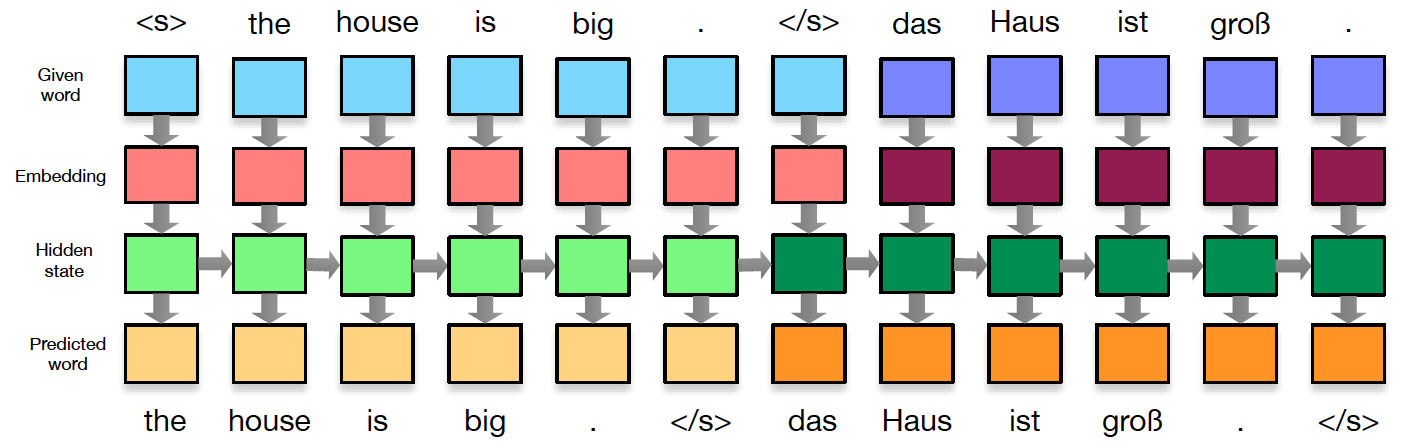
\includegraphics[scale=0.6]{seq2seq.png}
\caption{\label{fig:seq2seq}Sequence-to-sequence encoder-decoder model}
\end{figure} 

The task of the encoder is to provide a representation of source sentence or text. Then the representation of the decoded source will go through the predictions of the model which output an end of sentence token. During this process, the hidden state of the source actually encodes the meanings and the vector which hold the values before going through decoder is called the \textsl{input sentence embedding}. After the \textsl{encoder phase}, the hidden state will be decoded in the \textsl{decoder phase}. 

In decoder phase, the decoder should be able to predict the next word according to the information it can decode and also need to care about the coverage of the translation. So, the tasks of decoder cover two parts: prediction and translation.
  
\subsubsection{RNN Aligned Model}
Based on the previous encoder-decoder model, recurrent neural network(RNN) is aligned into the hidden state\cite{koehn2017neural}. As the Figure~\ref{fig:rnn}, the left word will be passed to right in the first RNN and to get the right context a right-to-left RNN is added. Such a model is called \textsl{bidirectional recurrent neural network}. Denote the left-to-right hidden state as $\overrightarrow{h}$ and right-to-left as $\overleftarrow{h}$, then the mathematical representation of these two RNN are:

$$
\begin{array}{rcl}
\overrightarrow{h_j}&=&f(\overrightarrow{h_{j+1}}, \bar{E} x_j)\\
\overleftarrow{h_j}&=&f(\overleftarrow{h_{j+1}}, \bar{E} x_j)
\end{array}
$$

where the $x_j$ denotes an input word and for the general mapping function $f$, it can be feed-forward neural network, more complex recurrent unit(GRUs) or Long short-term memory(LSTM).

\begin{figure}
\centering
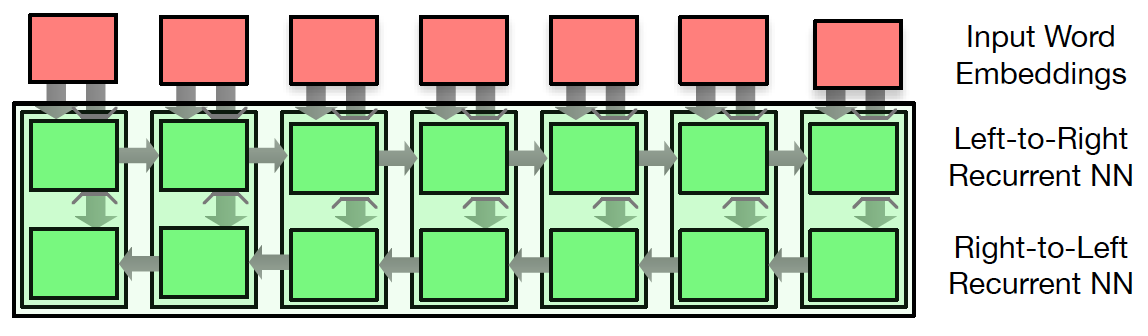
\includegraphics[scale=0.7]{rnn.png}
\caption{\label{fig:rnn}Input Encoder}
\end{figure}

Combined with hidden states, the decoder is also RNN(Figure~\ref{fig:rnn2}) which takes the representation of the input context, the hidden states, and the output of the prediction to generate new hidden decoder state as well as word predictions. 

The decoder will compute a sequence of hidden states $s_i$ from previous hidden state $s_{i-1}$, the embedding of the previous output word $Ey_{i-1}$, and the input source $c_i$, and it is defined as:

$$s_i = f(s_{i-1}, Ey_{i-1}, c_i)$$ 
 
The function here also has multiple choices including GRUs, and LSTM, and so on.

\begin{figure}
\centering
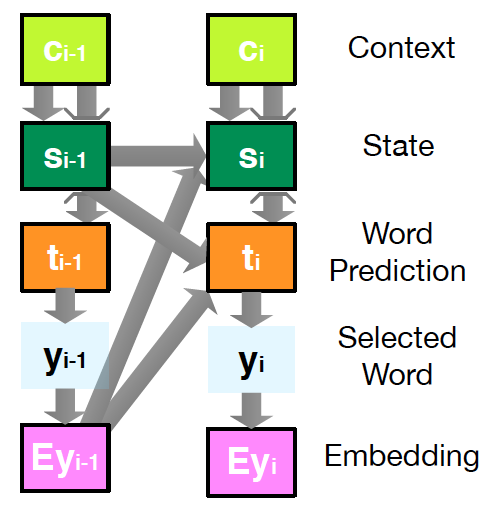
\includegraphics[scale=0.6]{rnn_2.png}
\caption{\label{fig:rnn2}Output Decoder}
\end{figure}

In Figure~\ref{fig:rnn2}, $t_i$ is a conditioned values on the decoder hidden state $s_{i-1}$. So, the embedding of the previous output word $Ey_{i-1}$ and the input text $c_i$ can be represented as 

$$t_i = \text{softmax}(W(U_{s_{i-1}}+VEy_{i-1}+Cc_i))$$

The softmax here can ensure the sum of the vector of the prediction probability be $1$ and the max value indicates the output $y_i$.

\subsubsection{Attention Based Model}
Attention is a mechanism of NMT, it enables NMT to use the most relevant parts of the source sentence at each translation step. Attention is different from the alignment in some cases and is capturing useful information other than alignments\cite{ghader2017does}. This ability makes attentional NMT models perform better in handling long sentences.

There are two popular attention models: \textsl{global attention model} and \textsl{local attention model}. Common of these two models is in each time step $t$, attention layer uses the hidden state of LSTM $\tilde{h}_t$ as input to derive a context vector. The difference of the two models is the way they compute the context vector. Figure~\ref{fig:attention1} and Figure~\ref{fig:attention2}\cite{luong2015effective} shows the difference.

\begin{figure}[H]
\centering
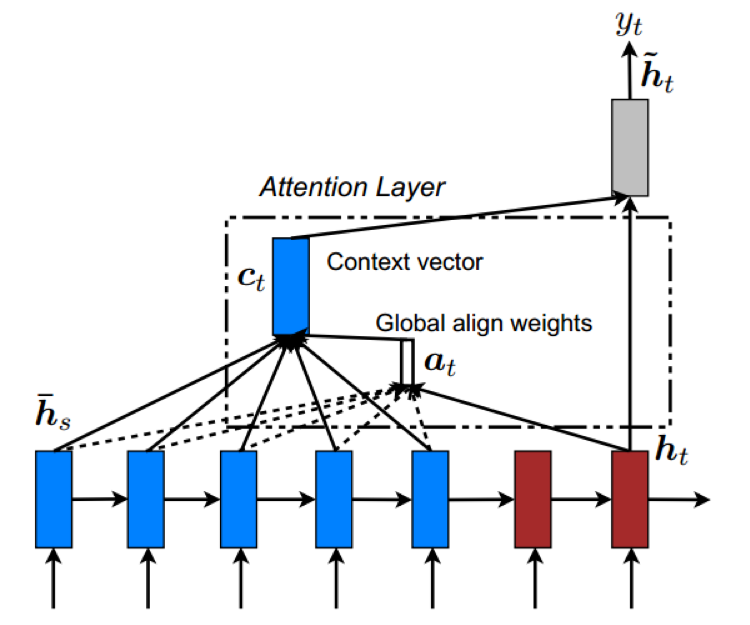
\includegraphics[scale=0.5]{attention_1.png}
\caption{\label{fig:attention1}Global Attention Model}
\end{figure}

\begin{figure}[H]
\centering
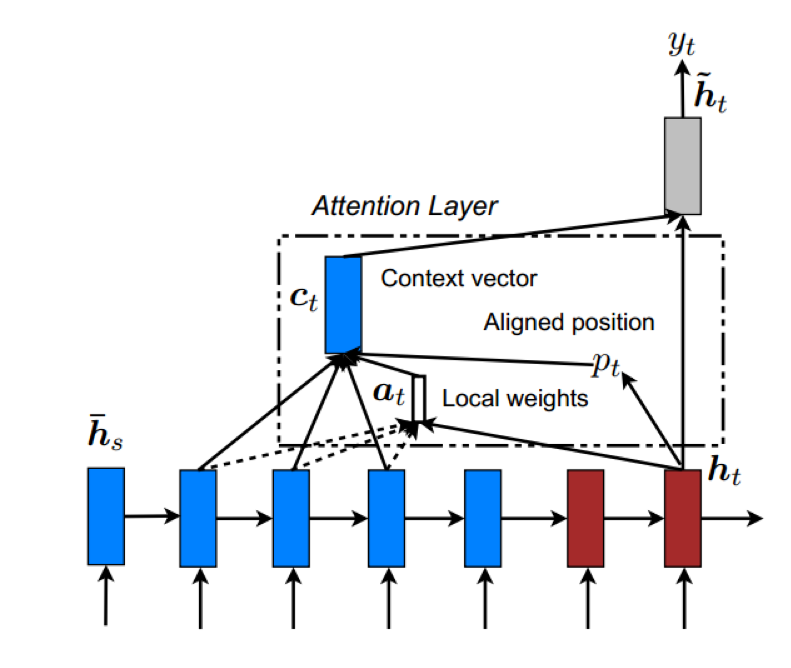
\includegraphics[scale=0.5]{attention_2.png}
\caption{\label{fig:attention2}Local Attention Model}
\end{figure}

In Figure~\ref{fig:attention1}, the global model infers a variable-length alignment weight vector at based on the current target state. In Figure~\ref{fig:attention2}, the local model first predicts a single aligned position for the current target word. A window centred around the source position is then used to compute a context vector. In global attention model, the attention layer focuses on the context of each word and the context vector contains the context information so that the model can use this information to perform better especially in translating long sentences.But if the sentence is much too long, the cost of calculation will be unacceptable. Thus, the local attention model is needed. Local attention model calculates the aligned position of each word first which gives the bound of the context of each word making the calculation of context vector easier.

\subsection{Techniques}
\subsubsection{Beam Search}
Beam search\cite{papineni2002bleu} is often used in statistical machine translation or neural machine translation to optimize the decoding process. In Figure~\ref{fig:beam}, assume that the beam length is $2$, that is, only $2$ search paths are reserved at a time, and the decoder needs to output $2$ target language words with the highest probability as candidates each time. And the decoder finally select the target language sequence with the highest probability as output.

\begin{figure}[H]
\centering
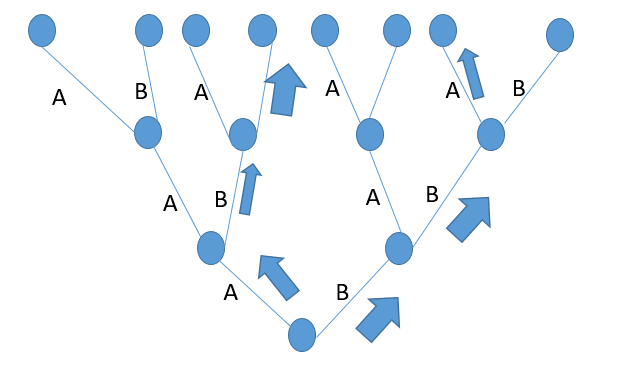
\includegraphics[scale=0.5]{beamsearch.png}
\caption{\label{fig:beam}Beam Search(Length $2$)}
\end{figure}

\subsubsection{Residual Connection}
Residual connection(Figure~\ref{fig:residual}) is a cross-level connection mechanism\cite{googleNMTS}. Adding an identity mapping to the original RNN network, the original output is integrated with the direct input as the output, slowing down the rate of gradient descent to achieve the purpose of deepening the number of layers in the RNN network and reducing the difficulty of training.

\begin{figure}[H]
\centering
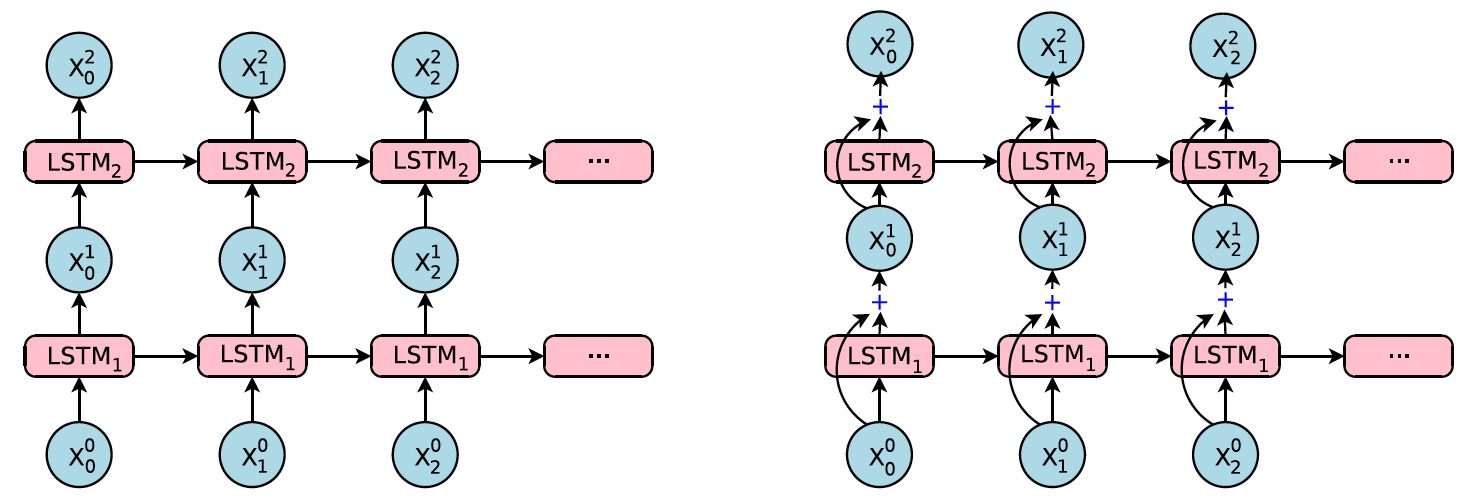
\includegraphics[scale=0.5]{residualconnection.png}
\caption{\label{fig:residual}The difference of LSTM and Google's LSTM with residual connection}
\end{figure}

\subsection{Example: Google's NMTS}
In \cite{googleNMTS}, Google's Neural Machine Translation System is a model consists of a deep LSTM with $8$ encoder and $8$ decoder layers using residual connection(Figure~\ref{fig:residual}) as well as attention connections from the decoder network to the encoder. As Figure~\ref{fig:googleNMTS} shows, this model can be divided into three parts: encoder, decoder and the attention work. The encoder will transform the source sentence into a list of vectors in which every vector is a input symbol. The decoder will produces one symbol each time till the special end-of-sentence(EOS) is produced. The attention network connects the encoder and the decoder and make the decoder can focus on various regions of the source.

\begin{figure}[H]
\centering
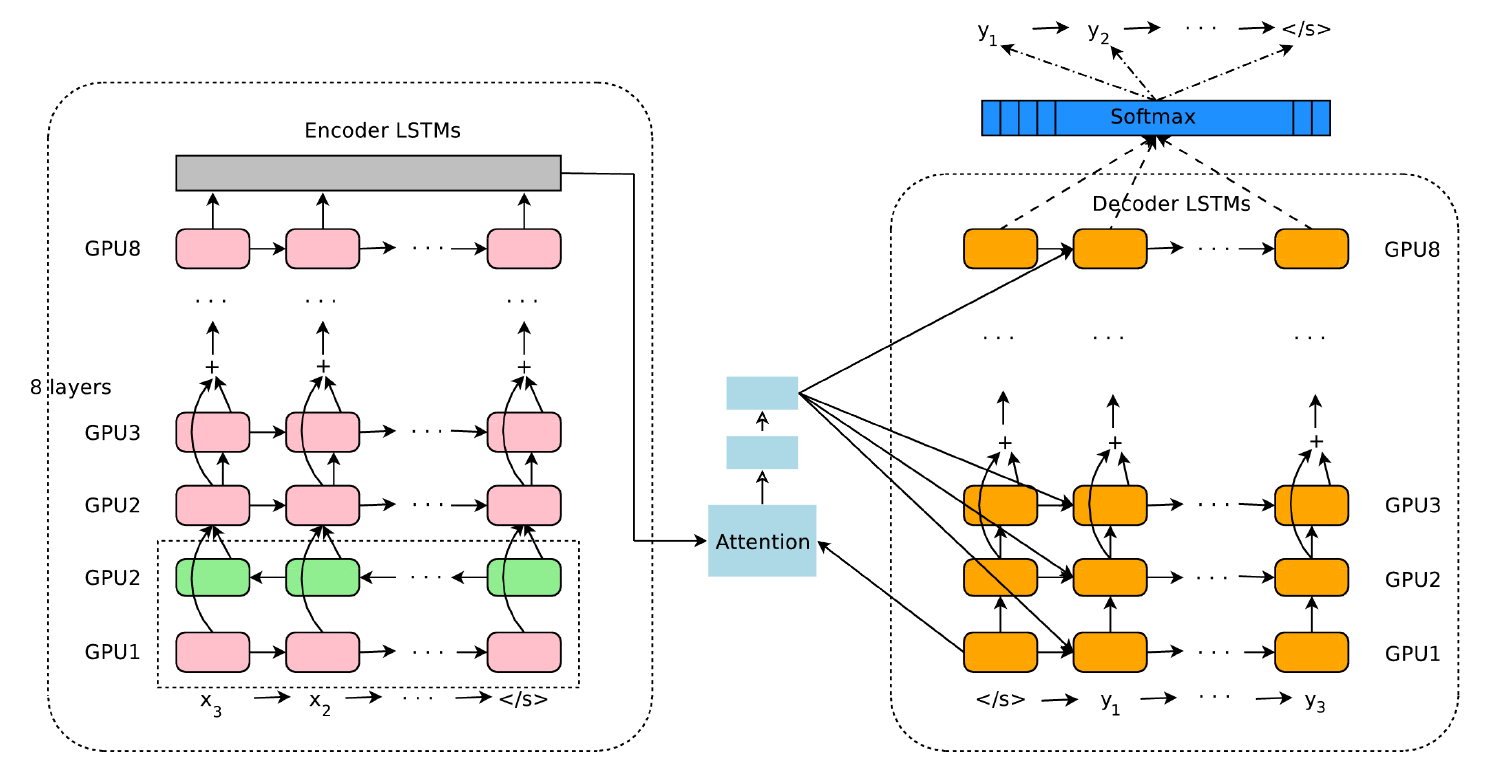
\includegraphics[scale=0.5]{googleNMTS.png}
\caption{\label{fig:googleNMTS}Google's Neural Machine Translation System}
\end{figure}

\subsection{Datasets}
Workshop on Statistical Machine Translation(WMT) is a widely used dataset post by Annual Meeting of the Association for Computational Linguistics. It contains training data, different tasks, and machine translation models. For example, in WMT 2018 eight language pairs are provided, along with a common framework. Its task is to improve current methods. Europarl is another widely used data set. It contains the data of parallel texts which are often from multinational institutions such as the United Nations, the European Union and the governments of multilingual countries. Europarl comprises of about 30 million words for each of the $11$ official European languages.

\begin{itemize}
	\item WMT Dataset
	
	The provided data is mainly taken from public data sources such as the Europarl corpus, and the UN corpus. Additional training data is taken from the News Commentary corpus.It allows participants to submit translations for any languages the data set contains.Human judges will judge the performance.The data has been divided into several tasks,including neural MT training task.This task requires the participants to train a fixed neural MT model with fixed data.Participants are required to submit the variables file i.e. the neural network.
	
	\url{http://www.statmt.org}	
	
	\item Europarl Dataset\cite{europarl}
    
    The Europarl parallel corpus is extracted from the proceedings of the European Parliament. It includes versions in $21$ European languages: Romanic (French, Italian, Spanish, Portuguese, Romanian), Germanic (English, Dutch, German, Danish, Swedish), Slavik (Bulgarian, Czech, Polish, Slovak, Slovene), Finni-Ugric (Finnish, Hungarian, Estonian), Baltic (Latvian, Lithuanian), and Greek.

	\url{http://www.statmt.org/europarl/}

	\item Linguistic Data Consortium(LDC)
	
	The Linguistic Data Consortium (LDC) is an open consortium of universities, libraries, corporations and government research laboratories. LDC initially was a repository and distribution point for language resources. With the development of the LDC, it then changed to be an organization and nowadays it supports language resources for language-based technology evaluations.
	
	\url{https://www.ldc.upenn.edu}

	\item OPUS\cite{TIEDEMANN12.463}
	
	OPUS is a growing collection of translated texts from the web. The main Chinese dataset is \textsl{MultiUN} and \textsl{OpenSubtitles2016}.
	
	\url{http://opus.lingfil.uu.se/MultiUN.php}	
	
	\url{http://opus.lingfil.uu.se/OpenSubtitles2016.php}	

	\url{http://opus.lingfil.uu.se/}	
		
	\item Acquis Communautaire(AC)
	
	As there were $20$ official EU languages at the beginning of the year 2005, the AC thus exists as a parallel text (text and its translation) in $20$ languages. The languages are Czech, Danish, German, Greek, English, Spanish, Estonian, Finnish, French, Hungarian, Italian, Lithuanian, Latvian, Maltese, Dutch, Polish, Portuguese, Slovak, Slovene and Swedish.
	
	\url{https://wt-public.emm4u.eu/Acquis/JRC-Acquis.2.2/doc/README_Acquis-Communautaire-corpus_JRC.html}	
	
	\item UM-Corpus\cite{tian2014corpus}
	
	The UM-Corpus has been designed to be a multi-domain and balanced parallel corpus for research and development purpose. In this version, a two million English-Chinese aligned corpus is provided, and it is categorized into eight different text domains, covering several topics and text genres, including: Education, Laws, Microblog, News, Science, Spoken, Subtitles, and Thesis.	
	
	\url{http://nlp2ct.cis.umac.mo/um-corpus/index.html}
	
\end{itemize}

\subsection{Evaluation}
\subsubsection{Bilingual Evaluation Understudy(BLEU)}
The essence of \textsl{BLEU} is the calculation of the co-occurrence frequency of two sentences\cite{papineni2002bleu}. BLEU's design philosophy is consistent with the idea of judging good or bad machine translation: The closer the machine translation results are to the results of professional human translation, the better. What the BLEU algorithm is actually doing: judging the similarity of two sentences. In the BLEU, If a machine translation is compared with its corresponding reference translation, a comprehensive score is calculated. The higher the score, the better the machine translates.

The process to compute the BLEU is that firstly compute $p_n$,
where $p_n$ is a modified precision score named modified $n$-gram precision. The molecular is the sum of the clipped $n$-gram counts for all the candidate sentences which appear in references and the denominator is the number of candidate $n$-grams in the test corpus.

$$p_n = \frac{\sum_{\mathcal{C}\in\{Candidates\}}\sum_{n-gram\in \mathcal{C}}Count_{clip}(n-gram)}{\sum_{\mathcal{C'}\in\{Candidates\}}\sum_{n-gram'\in \mathcal{C'}}Count_{clip}(n-gram')}$$

Let $c$ be the length of the candidate translation and $r$ be the effective reference corpus length. It compares the length of the candidates and the references. Compute the brevity penalty BP:

\begin{equation}
BP=
\begin{cases}
1 & \text{if $c > r$}\\
e^{(1-r/c)} & \text{if $c \leq r$}
\end{cases}
\end{equation}

$BP$ can resolve the problem of judging whether the translation is complete.

Then, 

$$BLEU = BP \cdot \left(\sum_{n=1}^{N} w_n\log{p_n}\right)$$

BLEU value is calculated by combining the $p_n$ values corresponding to different lengths $n$.

If use the log domain, the ranking behaviour will more immediately apparent:

$$\log BLEU = \min{(1-\frac{r}{c}, 0)} + \sum_{n=1}^N w_n\log{p_n}$$

\subsection{Summary}
This part is a simplified survey including the basic model, a widely used technique and datasets of NMT. The model is very simple to understand in structure. RNN, LSTM are normally used to construct a deep neural network translation system. The attention mechanism is an important technique in NMT, two attention based models are introduced. For training ANN, the dataset is crucial and the well-known datasets are introduced. An evaluation BLEU is introduced since the measurement of model performance is a key point.

\section{Research Approach}


\subsection{Goal}
The goal of this project is an Android application which provides NMT through an off-line neural network. The application can accept users' voice and output corresponding translation results. The basic requirement of the translation service should include but not limit to Chinese-to-English and English-to-Chinese.

\subsection{Steps}
The process can be divided into steps:
\begin{enumerate}
	\item Target deep neural network models for NMT
	\item Adapt DNN model and deploy into application
	\item Test and optimize application on real mobile devices
\end{enumerate}

\subsection{Timeline}
The timeline of this this project can be referred as Figure~\ref{fig:timeline}.

\begin{figure}[H]
\centering
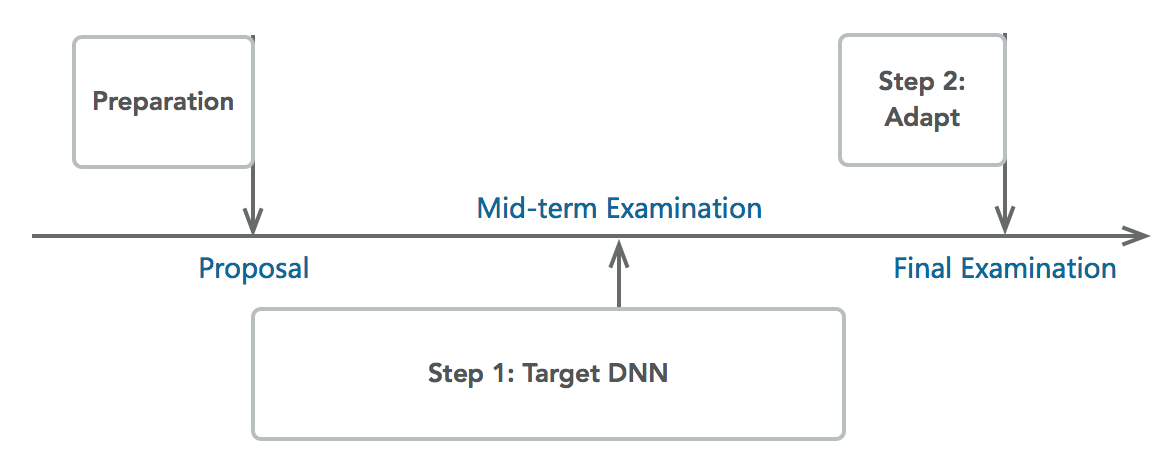
\includegraphics[scale=0.7]{timeline.png}
\caption{\label{fig:timeline}Timeline}
\end{figure}


\section{Technology Roadmap}
The rough roadmap of this project can be represent as Figure~\ref{fig:roadmap}

\begin{figure}[H]
\centering
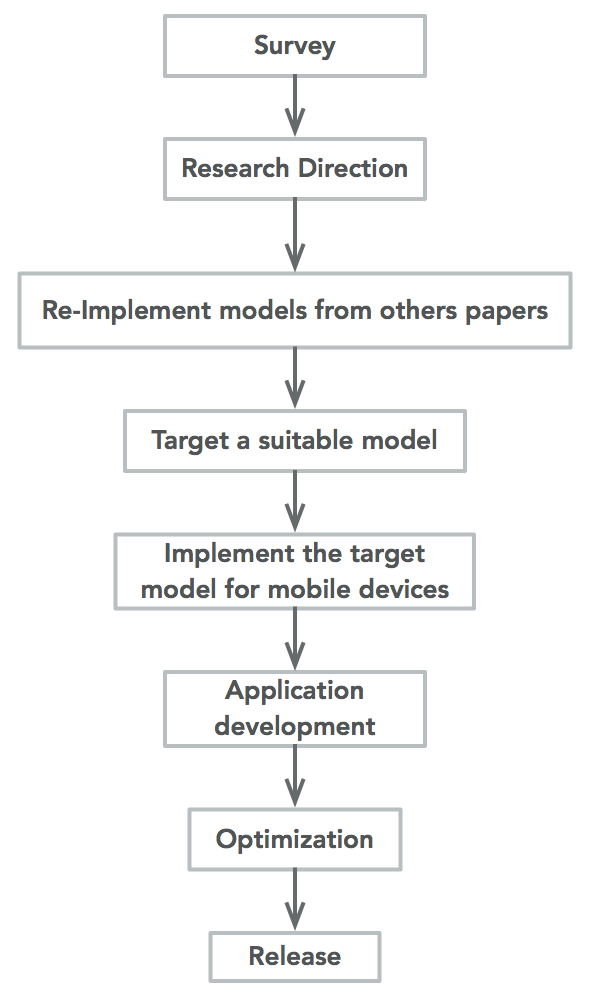
\includegraphics[scale=0.5]{roadmap.png}
\caption{\label{fig:roadmap}Technology Roadmap}
\end{figure} 

\section{Experiment Settings}
The first part is the core of this project is now our focus. After our primary research, we are going to reproduce the models in some papers we have read. Multiple datasets will be used to test various models and the best-performed model will be selected as the target model. After that, neural network compression will be the new challenge of our project, we will then focus on compressing our DNN model for mobile devices. The final model will be a compressed deep neural network model integrated into an Android application.

\section{Conclusion}
So far, we have already finished our primary research and have comprehended the basic model and method of NMT. NMT focuses on handling machine translation problem by using sequence handling ability of deep neural networks. We also have some understanding of models and techniques of NMT as well as the data set and its evaluation standard. In the future, we are going to choose one or more models and algorithms in the papers to reproduce. After then we will focus on Neural network compression to deploy the models on mobile devices. At last, we will combine our product with voice technology, so that our problem can be solved.

\appendix



\newpage
\bibliographystyle{plain}
\bibliography{biblist}



\end{document}